\documentclass[11pt]{article}
\usepackage[a4paper,margin=1in]{geometry}
\usepackage[utf8]{inputenc}
\usepackage[T1]{fontenc}
\usepackage{microtype}
\usepackage{amsmath,amssymb}
\usepackage{booktabs}
\usepackage{tikz}
\usepackage{pgfplots}
\pgfplotsset{compat=1.18}
\usepackage[hidelinks]{hyperref}

\title{\textbf{The Test the Metaphor Benchmark Never Ran}}
\author{Vasili Gavrilov\thanks{Independent researcher. The pre-registration, every script,
and the audit's C driver: \url{https://github.com/Anode1/cjitter}; the data is the
benchmark's own release, Zenodo 10.5281/zenodo.10561215.}}
\date{Draft, August 2026}

\begin{document}
\maketitle

\begin{abstract}
The largest benchmark of metaphor-based optimization heuristics ran 294 implementations
for 1{,}411{,}200 runs on the 24 BBOB functions and ranked them by anytime performance.
It contains no statistical test: the word appears once, in a reference title, and none of
the 21 papers citing it adds one. Its raw data is public, and the missing test is
computable from it. We pair every implementation with random search per function,
instance and repetition at the benchmark's own budgets, apply the exact one-sided sign
test, and correct with Holm across the 296 implementations its release contains. At the
top budget of $10^4 d$ evaluations, 66 to 98 implementations per dimension, one in three
in 2D, are not shown better than uniform random sampling at equal cost, and 53 to 79 of
those are shown strictly worse. The count of implementations worse than random rises
toward the top budget in every dimension: a search that stalls loses ground to a
control that keeps sampling. The verdicts barely depend on the
control's distribution, 121 of 7{,}104 change between the benchmark's own random search
and a true uniform control. They depend on the implementation: the same algorithm name
carries opposite verdicts across libraries in eight of the cases where a name appears
twice, differential evolution among them. The audit is pre-registered, byte-reproducible,
and one program run against the benchmark's own release.
\end{abstract}

\section{A million runs and no test}

Vermetten, Doerr, Wang, Kononova and B\"ack \cite{vermetten24} benchmarked the
metaphor-heavy optimization libraries at a scale nobody had attempted: 294
implementations from mealpy, Opytimizer, NiaPy and EvoloPy plus twelve baselines, the 24
noiseless BBOB functions \cite{coco}, dimensions 2, 5, 10 and 20, ten instances, five
repetitions, $10^4 d$ evaluations each, collected with IOHexperimenter \cite{ioh}. The
paper ranks by an anytime measure and observes, among much else, that random search
beats over 30\% of the implementations on one function. It draws no statistical
conclusion, because it computes no test.

That is not a criticism of the collection; it is the opening the collection leaves. The
polemic against metaphor methods has run for a decade on S\"orensen's terms
\cite{sorensen15}, and the one quantitative reply a practitioner needs is still per
implementation: at my budget, does this method beat drawing points at random, or not?
The benchmark's release \cite{zenodo} carries every run, so the question has an exact
answer that requires no new optimization run at all. This paper computes it.

\section{The data and the two controls}

The release's processed fixed-budget files carry, per implementation, function, instance
and repetition, the best error reached by budgets $b \cdot d$ for
$b \in \{10, 50, 100, 500, 1000, 5000, 10000\}$. We audit what the release contains: 296
implementations across the four libraries (14 EvoloPy, 53 NiaPy, 82 Opytimizer, 147
mealpy) beside the twelve baselines; the paper's own count is 282, and the difference is
a property of the release we report rather than resolve. 278 of the 296 have the full
$24 \times 10 \times 5 = 1200$ runs per dimension; the other 18 are audited on the runs
present, 19 pairs in the worst case, with coverage printed beside every verdict.

Two controls, because the benchmark's own is not what its name says. The release's
\texttt{RandomSearch} is nevergrad's: a Gaussian pushed through the bound transform
of a \texttt{set\_bounds} array, concentrated toward the centre of the box. The
second control is uniform on the box, drawn by our own library's control method through
the COCO C evaluator \cite{coco}, same functions, instances, dimensions, budget grid and
repetition count, deterministic from declared seeds. The two evaluators agree to
$7 \times 10^{-10}$ on 180 probe points, so pairing across them is sound.

\section{The test}

Within one (implementation, dimension, budget), every run is paired with the control's
run on the same function, instance and repetition index, 1200 pairs when coverage is
full. A strict error win counts for the implementation, a strict loss against it, a tie
for neither. Under the null that the implementation is no better than the control, wins
are at most a fair coin, and the exact one-sided binomial tail
$p = 2^{-n}\sum_{k \ge w}\binom{n}{k}$ is the sign test. We test both directions,
correct with Holm \cite{holm79} across the 296 implementations within each (dimension,
budget), separately per direction, and declare at 5\% after correction: \emph{better},
\emph{worse}, or \emph{not shown}, where not shown is a failure to demonstrate and is
never read as equality. The budget factor 10 is excluded by pre-registration: below most
population sizes the compared value is the shared-seed initial sample, and one baseline
has no data there. The design, families, tie rule and exclusions were frozen in a
pre-registration before any confirmatory number was computed, with the exploratory pilot
it followed disclosed inside it.

\section{What the audit finds}

Against the uniform control, per dimension at the top budget of $10^4 d$ evaluations:

\begin{center}\small
\begin{tabular}{lrrrr}
\toprule
 & $d=2$ & $d=5$ & $d=10$ & $d=20$ \\
\midrule
shown better than uniform sampling & 198 & 217 & 224 & 230 \\
not shown & 19 & 13 & 14 & 13 \\
shown worse & 79 & 66 & 58 & 53 \\
\midrule
not shown better, total & 98 & 79 & 72 & 66 \\
\bottomrule
\end{tabular}
\end{center}

One implementation in three in 2D, one in four or five in the higher dimensions, spends
$10^4 d$ evaluations without demonstrated advantage over drawing points uniformly at
random; the clear majority of those are strictly worse. Against the benchmark's own
random search the row reads 100, 79, 71, 65: the audit's verdicts are not an artifact of
the control's distribution, since only 121 of the 7{,}104 verdict cells change between
the two controls, most in 2D at the two smallest budgets.

\paragraph{Worse grows with budget.} Figure~\ref{fig:trend} has the counts. In 2D they
run 58, 69, 64, 64, 72, 79 across the six budget factors; in 5, 10 and 20 dimensions
the minimum sits in the middle of the grid, at $500d$ to $1000d$ evaluations. The mechanism is not subtle: uniform sampling
improves for as long as it runs, and an implementation that stalls, on a bound, on a
collapsed population, on its own attraction to the centre, is overtaken and then left
behind. A method can be honestly better than random at $500 d$ evaluations and honestly
worse at $10^4 d$.

\begin{figure}[t]\centering
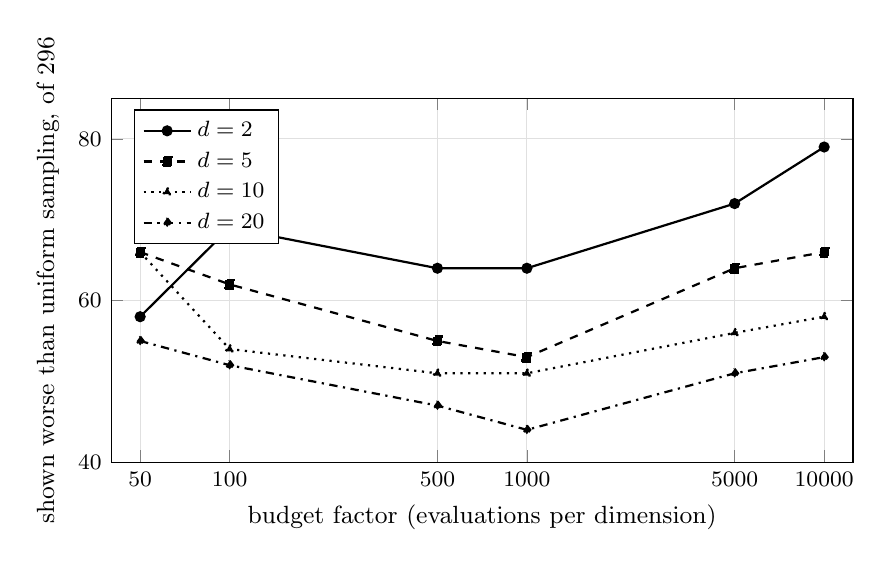
\begin{tikzpicture}
\begin{axis}[width=11cm,height=6.2cm,
  xmode=log,log basis x=10,
  xlabel={budget factor (evaluations per dimension)},
  ylabel={shown worse than uniform sampling, of 296},
  ymin=40,ymax=85,xmin=40,xmax=12500,
  xtick={50,100,500,1000,5000,10000},
  xticklabels={50,100,500,1000,5000,10000},
  legend pos=north west,legend cell align=left,
  grid=major,grid style={black!12},
  tick label style={font=\footnotesize},label style={font=\small},
  legend style={font=\footnotesize}]
\addplot[thick,mark=*,mark size=1.6pt] coordinates
  {(50,58)(100,69)(500,64)(1000,64)(5000,72)(10000,79)};
\addlegendentry{$d=2$}
\addplot[thick,mark=square*,mark size=1.6pt,dashed] coordinates
  {(50,66)(100,62)(500,55)(1000,53)(5000,64)(10000,66)};
\addlegendentry{$d=5$}
\addplot[thick,mark=triangle*,mark size=1.6pt,dotted] coordinates
  {(50,66)(100,54)(500,51)(1000,51)(5000,56)(10000,58)};
\addlegendentry{$d=10$}
\addplot[thick,mark=diamond*,mark size=1.6pt,dashdotted] coordinates
  {(50,55)(100,52)(500,47)(1000,44)(5000,51)(10000,53)};
\addlegendentry{$d=20$}
\end{axis}
\end{tikzpicture}
\caption{Implementations shown strictly worse than uniform sampling at equal budget,
of 296, exact sign test with Holm at 5\% per (dimension, budget). The count rises
toward the top budget in every dimension, from a mid-grid minimum in 5, 10 and 20
dimensions: a search that stalls is overtaken by a control that keeps sampling.}
\label{fig:trend}
\end{figure}


\paragraph{The implementation, not the metaphor.} Eleven algorithm names appear in two
or more libraries. At the top budget the verdict disagrees across libraries for eight
(name, dimension) cells: mealpy's \texttt{DE} is shown worse than uniform sampling in
all four dimensions while EvoloPy's and Opytimizer's DE are shown better, and SCA splits
the same way between Opytimizer (worse) and EvoloPy (better). Differential evolution is
not a metaphor method, which is the point: the audited unit is a shipped implementation,
and a verdict attaches to code, not to the idea the code is named after.

\paragraph{Effect sizes.} Beside each verdict we report the median over pairs of the
error ratio implementation over control. At the top budget the median metaphor
implementation delivers 5 to 28 per cent of uniform sampling's error, a real advantage;
the upper quartile sits at 0.89 to 1.63, at or behind the control; the tails run from
$10^3$ times better to $3.8 \times 10^3$ times worse in 2D.

\paragraph{Checks.} The audit's own controls behaved: differential evolution, the two
modular CMA variants, L-SHADE and BIPOP are shown better in every dimension at the top
budget, with win rates of 1131 to 1200 out of 1200. One baseline anomaly is
pre-registered for verification against the raw logs and reported in
Section~\ref{sec:threats}.

\section{What this does and does not say}\label{sec:threats}

\textbf{BBOB is shifted and rotated.} Kudela \cite{kudela} showed that several
metaphor methods, grey wolf and whale among them, concentrate their search at the centre
of the box and collapse when the optimum moves. BBOB moves it by construction. So a
worse-than-random verdict here is a verdict about behaviour on shifted problems, a
published failure mode, and the audit's claim is exactly "not shown better than random
sampling on this benchmark at these budgets", never "worthless everywhere". The
near-identity of the two controls' verdicts adds one fact to that discussion: the
centre-concentration of the benchmark's own baseline moved almost nothing.

\textbf{The nevergrad PSO anomaly.} The release's own \texttt{ng\_PSO} baseline is shown
worse than random in 10 and 20 dimensions at every budget, 35 wins of 1200 at the 10D
top budget. As pre-registered, the row was re-derived from the raw IOHprofiler logs in
the release before being stated: 105 fixed-budget values across three cells,
differential evolution's among them, match the processed data to the digit, and the
anomaly is the implementation's own. On the 10D sphere its five runs end at errors of
18.6 to 34.6 after $10^5$ evaluations. The audit reads baselines and metaphors with the
same test, and this row is the demonstration.

\textbf{Coverage.} Eighteen implementations have incomplete panels in the release,
consistent with its Readme's warning about split raw folders; they are audited on the
pairs present and marked. A sensitivity pass restricted to complete 1200-pair cells
changes exactly one verdict anywhere in the confirmatory grid, a borderline not shown
that becomes better when the Holm family shrinks (mealpy's ImprovedSFO, 5D, budget
$5000d$, corrected $p$ crossing at 0.049), and no cell of the top-budget table; every
other count falls exactly by the excluded rows' own verdicts.

\textbf{One benchmark, one budget grid.} Nothing here transfers to constrained, discrete
or expensive problems, and a method not shown better at $10^4 d$ may be the right tool
at $10 d$: the budget trend above is the demonstration.

\section{The instrument}

The tests are two public functions of a small C library, \texttt{cjitter\_sign\_p} and
\texttt{cjitter\_holm}, the same two its comparison harness uses to judge its own four
search methods against a matched-budget uniform control; the audit's driver reads the
release's runs and prints every verdict in this paper in 18 seconds; the full verdict
tables under both controls ship beside this paper in \texttt{audit-data/}. The library exists
because the comparison discipline used here, a control at equal budget, paired seeds,
an exact test, a declared family, is cheap enough to live inside an API rather than in a
paper's methods section.

Auditing at this scale repaired the instrument once: the exact binomial tail, summed as
plain doubles, overflows $\binom{n}{k}$ past $n = 1028$ and returned NaN on the first
1200-pair panel. The shipped sum now carries an exact power-of-two scale, changes no
byte of any smaller panel, and is pinned against exact rational references. An audit
tool that had never met a pooled panel would have printed nothing wrong and nothing at
all; the failure surfaced because the tests pin values, which is the discipline this
paper is asking benchmarks to adopt.

\begin{thebibliography}{9}
\bibitem{vermetten24} D.~Vermetten, C.~Doerr, H.~Wang, A.~V. Kononova, T.~B\"ack.
Large-Scale Benchmarking of Metaphor-Based Optimization Heuristics. In \emph{GECCO
2024}, 41--49. DOI 10.1145/3638529.3654122.
\bibitem{zenodo} D.~Vermetten et al. Reproducibility files for \cite{vermetten24}.
Zenodo, DOI 10.5281/zenodo.10561215, CC-BY 4.0.
\bibitem{sorensen15} K.~S\"orensen. Metaheuristics---the Metaphor Exposed.
\emph{International Transactions in Operational Research} 22(1):3--18, 2015.
\bibitem{kudela} J.~Kudela. The Evolutionary Computation Methods No One Should Use.
arXiv:2301.01984, 2023.
\bibitem{holm79} S.~Holm. A Simple Sequentially Rejective Multiple Test Procedure.
\emph{Scandinavian Journal of Statistics} 6(2):65--70, 1979.
\bibitem{coco} N.~Hansen, A.~Auger, R.~Ros, O.~Mersmann, T.~Tu\v{s}ar, D.~Brockhoff.
COCO: A Platform for Comparing Continuous Optimizers in a Black-Box Setting.
\emph{Optimization Methods and Software} 36(1):114--144, 2021.
\bibitem{ioh} J.~de~Nobel, F.~Ye, D.~Vermetten, H.~Wang, C.~Doerr, T.~B\"ack.
IOHexperimenter: Benchmarking Platform for Iterative Optimization Heuristics.
\emph{Evolutionary Computation} 32:205--210, 2024.
\end{thebibliography}

\end{document}
